\chapter*{Appendices}
\addcontentsline{toc}{chapter}{Appendices}

\appendix

\chapter{The celestial sphere and astronomical coordinates}
\label{app:coord}

\section{A place on Earth}

The terrestrial equator is defined as the great circle halfway between
the North and the South Poles.  The ``Prime Meridian'' was defined in
1884 as the half circle passing through the poles and the old Royal
Observatory in Greenwich, England (see Fig.~\ref{figearth}).

A location on the surface of the Earth is defined by three numbers:
the longitude $\lambda$, the latitude $\phi$, and the height above sea
level, $h$.

The longitude of a given point on Earth is measured westward from
Prime Meridian to the intersection with the equator of the circle of
longitude that passes through the point.

The latitude is the angle measured northward (positive) or southward
(negative) along the circle of longitude from the equator to the
point.

Onsala Space Observatory is located just a few meters above sea level,
at the following longitude and latitude:

\begin{center}
${\bf{\boxed{\lambda=12^{\circ}01'00'' \text{E}
\hspace{1cm}\phi=57^{\circ}25'00''\text{N.} }}}$
\end{center}  

\begin{figure}[ht]
\begin{center}
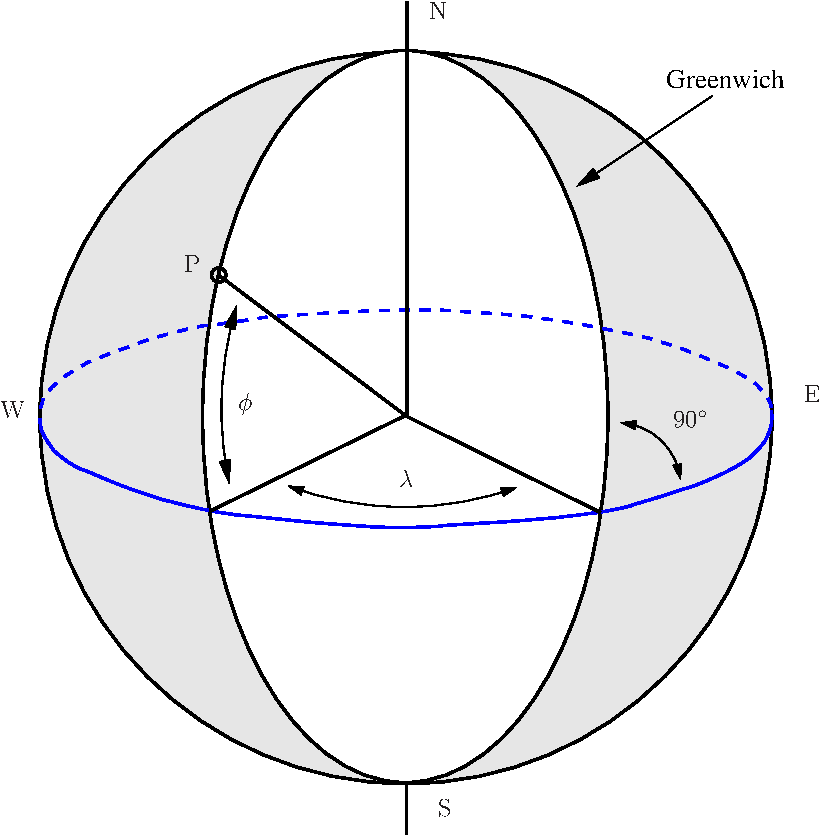
\includegraphics[width=8cm]{../figures/longlat.pdf}
\end{center}
\caption{Illustration of the terrestrial system, with longitude
  ($\lambda$) and latitude ($\phi$).  Great circles passing through
  the poles are circles of longitude.  Circles parallel to the Earth
  equator are circles of latitude. }
\label{figearth}
\end{figure}


\section{The celestial sphere}

\subsection{Equatorial coordinates}

\begin{figure}[ht]
\begin{center}
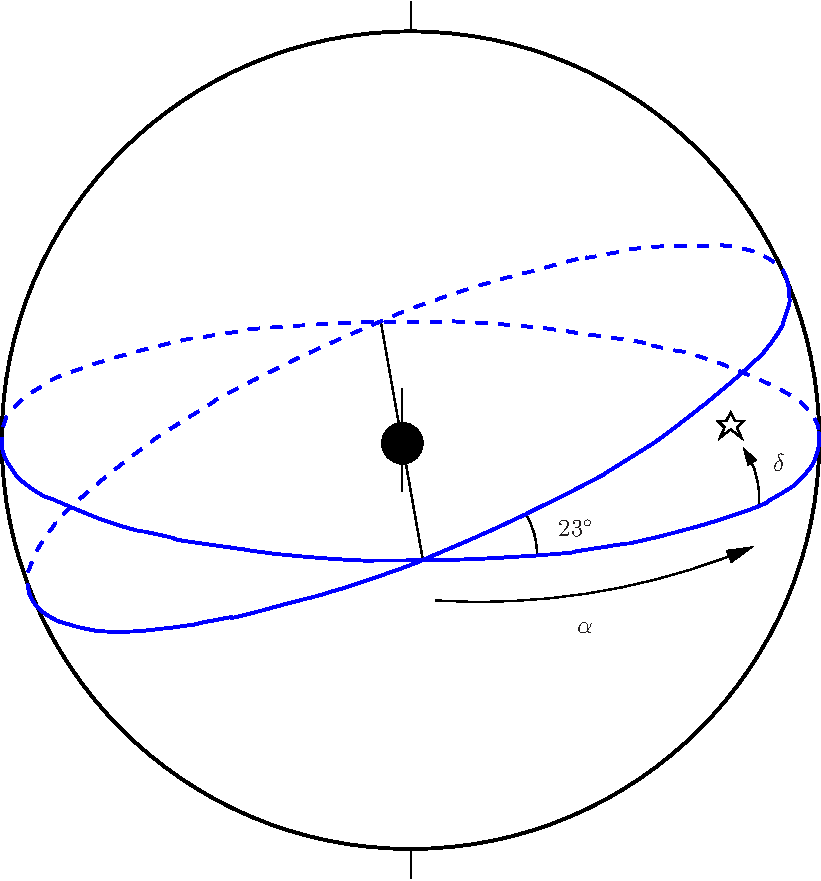
\includegraphics[width=8cm]{../figures/celestial.pdf}
\end{center}
\caption{Illustration of the celestial coordinate system, with right ascension $\alpha$ 
and declination $\delta$. 
Earth is at the center. The plane of the ecliptic is inclined by 23.5$^\circ$ with 
respect to the celestial equator. }
\label{figcelest}
\end{figure}

The celestial sphere is an imaginary sphere concentric with the Earth, on which
astronomical objects appear (see Fig.~\ref{figcelest}). 
The celestial equator is the
natural extension of Earth's equator. Because of the inclination of 
Earth's axis of rotation, the apparent annual path of the Sun
on the celestial sphere (the {\em ecliptic}) doesn't  coincide with the 
celestial equator; the ecliptic makes an angle of 23.5$^\circ$
with the celestial equator. The point where the Sun crosses the
celestial
equator going northward in spring is called {\bf the Vernal 
Equinox}. 
On the equinox, the Sun lies
in the Earth's equatorial plane, and the day and night are equally
long. The solstices mark the dates when the Sun is farthest from 
the celestial equator and occur around June~21 and December~21. 

\medskip
{\bf{$\rightarrow$ Mark the north and south celestial poles, 
the celestial equator, the ecliptic,
the solstices and the equinoxes on Fig.~\ref{figcelest}.}}
\medskip

Positions on the celestial sphere are defined by angles along 
great circles. By analogy with terrestrial longitude, 
right ascension (RA), $\alpha$, is the celestial longitude of an
astronomical object, 
but it is measured {\em eastward} from the Vernal Equinox
along the celestial equator. RA is expressed
in hours and minutes of time, with 24 hours corresponding 
to 360$^\circ$. 

In analogy with terrestrial latitude, declination (DEC), $\delta$, 
is the angular distance of an object from the celestial equator. 
Right ascension and declination $(\alpha,\delta)$ specify completely
a position on the celestial sphere. 

Imagine now that we find ourselves at location $P$ on Earth at a 
latitude $\phi$, and we want to observe the sky. 
An astronomical object
of declination $\delta$ reaches a maximum altitude above
the horizon, $h_{\rm max}$, and a minimum altitude, $h_{\rm min}$,
given by
\begin{equation}
\begin{array}{l}
h_{\rm max} = 90^\circ -|\phi-\delta| \\
h_{\rm min} = -90^\circ +|\phi+\delta|. 
\end{array}
\end{equation}

{\bf{$\rightarrow$ In Onsala, astronomical objects with $\delta > 33^\circ$
always remain above the horizon (they are circumpolar); those with $\delta <
-33^\circ$ never rise above the horizon.}}


\subsection{The Local Sidereal Time}

\begin{figure}[ht]
\begin{center}
 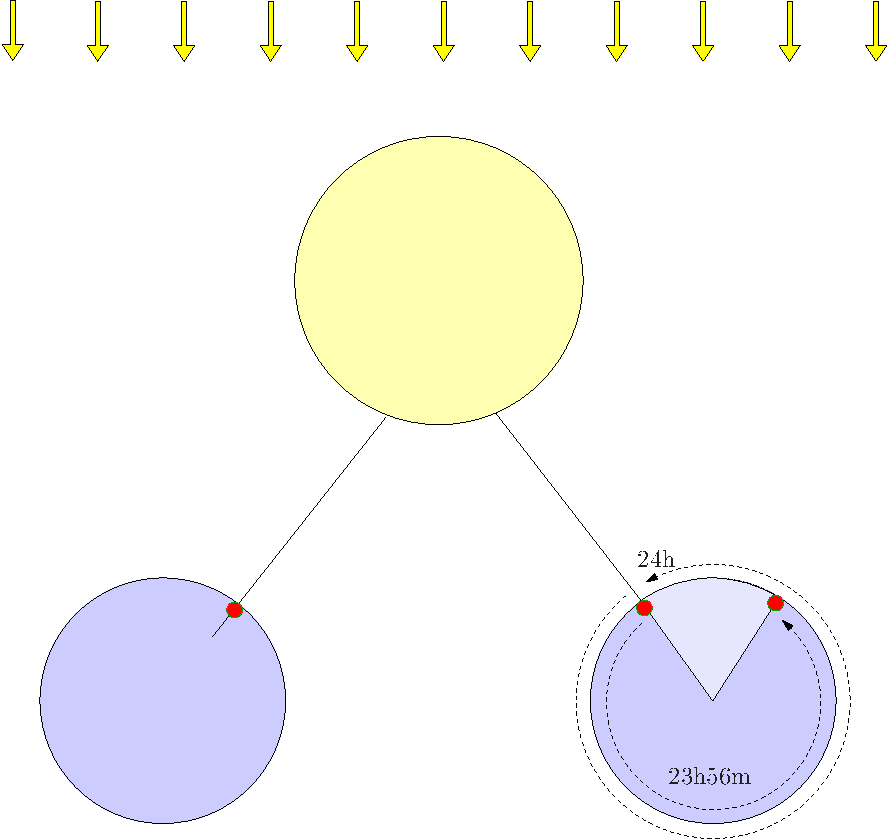
\includegraphics[width=8cm]{../figures/lst.pdf}
\end{center}
\caption{The Local Sidereal Time is the time relative to the stars, whereas the 
solar time is relative to the Sun. 24~hours of LST time pass in only 
23~hours 56~minutes 05~seconds of solar time, because Earth, having 
moved on its orbit around the Sun, finds itself the next day at the same position 
relative the stars {\em a bit earlier} than at the same position relative
to the Sun. 
In one year (365 days), Earth has moved 360$^\circ$ around the Sun and lost one 
turn (24 hours) relative to the stars. So the difference in one month is 2 hours, and in one day it is 24~hours/365 = 
3m56s.
}
\label{figlst}
\end{figure}

The convention of measuring RA eastward was chosen
because it makes the celestial sphere into the face of a clock. 
The hand of the clock is {\bf the local meridian}, 
the north-south line passing through the observer's zenith 
(the zenith is the upward prolongation of the observer's plumb line --
right overhead!). 

When the Vernal Equinox is on the local meridian, the Local Sidereal
Time (LST), or star time, is said to be 0 hours. 
On the Spring equinox (around March 21), this happens at noon (solar clock). 

{\bf$\rightarrow$ To remember: On the Spring equinox (around March~21), LST= 0~h at noon (solar time).}

As time passes, 
astronomical objects on the local meridian will have a larger RA.
At any moment and any location on Earth, 
the LST equals the RA of astronomical objects on the
local meridian. 

The celestial clock moves ahead of the solar clock every day. This 
is because Earth rotates both around its own axis, and also around the
Sun, as illustrated in Fig.~\ref{figlst}. 
After 24~hours of solar time, a given location on Earth 
finds itself at the same solar time (which is with respect to the Sun). 
For instance, every day the Sun reaches its highest elevation at the same 
solar time. 
But relative to the stars, it finds itself on 
the same position a little bit earlier (corresponding
to only one rotation around its axis). 24~hours of LST time
pass in only 
23 hours 56 minutes 05 seconds of solar time. A certain LST time
occurs about 4 minutes earlier than it had the day before. 

We have said that on the Spring equinox, around March 21, the LST is 0~h
at 12~h solar time (noon). The next day at noon, 
the LST will be 0 h 3 min and 56 sec; inversely, 0~h of LST time
correspond to 11~h 46~m 05~s solar time. 
With each passing month, a given LST time occurs 2~hours earlier. 

\subsection{How can I know whether my source is up?}
\label{app:visiblecoords}

Let's imagine that we want to observe in a certain direction in the
Galactic plane (a certain Galactic longitude $l$, and a Galactic 
latitude $b=0$) at a certain time. 

First of all, we need to convert the Galactic coordinates into 
celestial equatorial coordinates: RA and DEC. For this, we may use
the table to find $\alpha$ and $\delta$. 

As we have shown above, some sources will never rise above the horizon in Onsala 
(the ones with $\delta < -33^\circ$).   

It is best to study examples 
to learn how to find out when a source is visible. 

\bigskip
{\bf Example~1.} I have been allocated time to observe with the radio telescope
on May~5, starting at 15~hours local time in Onsala.  
This corresponds to 13~hours solar time. 
What is the corresponding LST time? What part of the Galaxy can I observe? 

\smallskip
On March 21, LST=0~h at noon. 

$\Rightarrow$ LST= 1~h at 13~h. 

May~5 occurs 1.5 months after March~21. The LST time shifts by
24 hours per year, or 2 hours per month. So, 1.5~months after
March~21, LST=1~h will occur at $=13 -(1.5\times 2) = 10$~h. 
And at 13~h, LST= 4~h. This means that sources will $\alpha=4$~h
will cross their meridian (be highest above the horizon) 
at that time.  

Looking at the table, we see that $l\simeq 150^\circ$ corresponds to $\alpha\simeq 4$~h. 
Since that Galactic longitude doesn't reach a very high elevation in Onsala, it is a 
good idea to start by observing it because it will be setting quickly. 

\bigskip
{\bf Example~2.} Today is Christmas Eve (December 24), and I have been offered a small optical
telescope. I would like to use it to observe the beautiful Whirlpool galaxy M~51. 
Is it possible? 

\smallskip
The coordinates of M~51 are $\alpha\simeq13$~h~30m, $\delta\simeq+47^\circ$. 
This means that M~51 will be at its highest elevation above the horizon at
LST=13~h~30. 

LST= 0~h at noon = 12~h around March~21. 

LST= 0~h at $12-(2\times 9) = -6$~h (or $24-6=18$~h) around Dec. 21 (9 months after March~21, 
since the LST time shifts ahead by 2 hours every month). 

LST=13~h~30 at 18+13~h~30= 7~h~30.  

M~51 will be highest up on the sky in the morning at 7~h30, and it will be rising during the
second part of the night. 




\begin{table}
\label{tabcoord}
\begin{center}
\begin{tabular}{rrr}
\hline
\medskip
$l$ & $\alpha(J2000)$ &$\delta(J2000)$\\
$^\circ$ &h m &$^\circ\,\,\,\,\,$$'$\\
\hline
0 & 17h45 & --28:56 \\
20 & 18h27 & --11:29 \\
40 & 19h04 & 06:17 \\
60 & 19h43 & 23:53 \\
{\bf\green 80}  & 20h35 & 40:39\\
{\bf\green 100} & 22h00 & 55:02\\
{\bf\green 120} & 00h25 & 62:43 \\
{\bf\green 140} & 03h07 & 58:17 \\
{\bf\green 160} & 04h46 & 45:14\\
180 & 05h45 & 28:56\\
200 & 06h27 & 11:29\\
220 & 07h04 & --06:17\\
240 & 07h43 & --23:53\\
\red 260 & 08h35 & --40:39\\
\red 280 & 10h00 & --55:02\\
\red 300 & 12h25 & --62:43\\
\red 320 & 15h07 & --58:17\\
\red 340 & 16h46 & --45:14\\
\hline
\end{tabular}
\caption{Conversion from Galactic coordinates to right ascension and
  declination for different values of $l$, with $b=0$.  The Galactic
  longitudes in bold face (and green) are circumpolar at the latitude
  of Onsala ($\delta > 33^\circ$).  The Galactic longitudes in red are
  always below the horizon at the latitude of Onsala.  }
\end{center}
\end{table}
